\documentclass[13pt]{beamer}
%
% Choose how your presentation looks.
%
% For more themes, color themes and font themes, see:
% http://deic.uab.es/~iblanes/beamer_gallery/index_by_theme.html
%
\mode<presentation>
{
\usetheme{CambridgeUS}     % or try Darmstadt, Madrid, Warsaw, ...
\usecolortheme{beaver} % or try albatross, beaver, crane, ...
\usefonttheme{default}  % or try serif, structurebold, ...
\setbeamertemplate{navigation symbols}{}
\setbeamertemplate{caption}[numbered]
} 

\usepackage[english]{babel}
\usepackage[utf8x]{inputenc}
\usepackage{xcolor}
\usepackage{multicol}
\usepackage{tikz}
\usepackage{tikz-uml}
\tikzumlset{font=\footnotesize\ttfamily}
\usepackage{hyperref}

\usepackage{listings}
\definecolor{codegreen}{rgb}{0,0.6,0}
\definecolor{codegray}{rgb}{0.5,0.5,0.5}
\definecolor{codepurple}{rgb}{0.58,0,0.82}
\definecolor{backcolour}{rgb}{0.95,0.95,0.92}

\lstdefinestyle{myCustomCppStyle}{
language=C++,
numbers=left,
stepnumber=1,
numbersep=9pt,
tabsize=2,
showspaces=false,
showstringspaces=false
}

\lstset{basicstyle=\tiny,style=myCustomCppStyle}

\lstdefinestyle{mystyle}{
backgroundcolor=\color{backcolour},   
commentstyle=\color{codegreen},
keywordstyle=\color{magenta},
numberstyle=\tiny\color{codegray},
stringstyle=\color{codepurple},
basicstyle=\ttfamily\footnotesize,
breakatwhitespace=false,         
breaklines=true,                 
captionpos=b,                    
keepspaces=true,                 
numbers=left,                    
numbersep=5pt,                  
showspaces=false,                
showstringspaces=false,
showtabs=false,                  
tabsize=1
}

\lstset{style=mystyle}

\usepackage{graphicx}
\graphicspath{ {./images/} }

\usepackage{tikz}
\usetikzlibrary{decorations.text}
\usetikzlibrary{shapes.geometric, arrows, positioning, calc, matrix}

\tikzset{
basic box/.style={
shape=rectangle, rounded corners, align=center,
draw=#1, fill=#1!25},
header node/.style={
Minimum Width=header nodes,
font=\strut\Large\ttfamily,
text depth=+0pt,
fill=white, draw},
header/.style={%
inner ysep=+1.5em,
append after command={
\pgfextra{\let\TikZlastnode\tikzlastnode}
node [header node] (header-\TikZlastnode) at (\TikZlastnode.north) {#1}
node [span=(\TikZlastnode)(header-\TikZlastnode)] at (fit bounding box) (h-\TikZlastnode) {}
}
},
hv/.style={to path={-|(\tikztotarget)\tikztonodes}},
vh/.style={to path={|-(\tikztotarget)\tikztonodes}},
fat blue line/.style={ultra thick, blue}
}

\definecolor{mygray}{RGB}{208,208,208}
\definecolor{mymagenta}{RGB}{226,0,116}
\newcommand*{\mytextstyle}{\sffamily\Large\bfseries\color{black!85}}
\newcommand{\arcarrow}[3]{%
% inner radius, middle radius, outer radius, start angle,
% end angle, tip protusion angle, options, text
\pgfmathsetmacro{\rin}{1.7}
\pgfmathsetmacro{\rmid}{2.2}
\pgfmathsetmacro{\rout}{2.7}
\pgfmathsetmacro{\astart}{#1}
\pgfmathsetmacro{\aend}{#2}
\pgfmathsetmacro{\atip}{5}
\fill[mygray, very thick] (\astart+\atip:\rin)
                 arc (\astart+\atip:\aend:\rin)
-- (\aend-\atip:\rmid)
-- (\aend:\rout)   arc (\aend:\astart+\atip:\rout)
-- (\astart:\rmid) -- cycle;
\path[
decoration = {
 text along path,
 text = {|\mytextstyle|#3},
 text align = {align = center},
 raise = -1.0ex
},
decorate
](\astart+\atip:\rmid) arc (\astart+\atip:\aend+\atip:\rmid);
}
\title[Design Pattern]{Structural Design Pattern}
\author{Hung Tran}
\institute{Fpt software}
\date{\today}


\begin{document}

\begin{frame}
\titlepage
\end{frame}

% Uncomment these lines for an automatically generated outline.
\begin{frame}{Outline}
\tableofcontents
\end{frame}

\section{Structural Pattern Overview}

\begin{frame}{Structural Pattern Overview}
	\begin{center}
	\textcolor{blue}{\textbf{How classes and objects are composed to form larger structure.}}
	\end{center}
	\begin{itemize}
		\item \textbf{Adapter}: Convert the interface of a class into another interface.
		\item \textbf{Bridge}: Decouple an abstraction from its implementation.
		\item \textbf{Composite}: Compose objects into tree structure.
		\item \textbf{Decorator}: Attach additional responsibilities to an object dynamically.
		\item \textbf{Façade}: Provide a unified interface to a set of interfaces.
		\item \textbf{Flyweight}: Use sharing to support large numbers of fine-grained objects efficiently.
		\item \textbf{Proxy}: Provide a surrogate or placeholder for another object to control access to it.
	\end{itemize}
\end{frame}

\section{Proxy pattern}

\begin{frame}{Problem Statement}
	\begin{columns}[T]
		\begin{column}{.5\textwidth}
			\begin{center}
			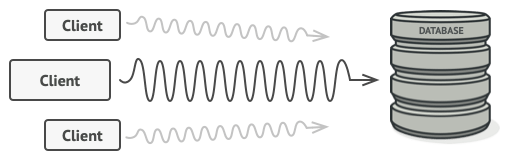
\includegraphics[scale=0.35]{./images/problem.png}
			\begin{itemize}
			\item In an ideal world, we’d want to put this code directly into our object’s class, but that isn’t always possible. For instance, the class may be part of a closed 3rd-party library.
			\end{itemize}
			\end{center}
		\end{column}
	
		\begin{column}{.5\textwidth}
			\begin{itemize}
				\item You have a massive object that consumes a vast amount of system resources. You need it from time to time, but not always.
				\item You could implement lazy initialization: create this object only when it’s actually needed.
				\item All of the object’s clients would need to execute some deferred initialization code. Unfortunately, this would probably cause a lot of code duplication.
			\end{itemize}
		\end{column}
	\end{columns}
\end{frame}

\begin{frame}{Solution: Facade Pattern}
	\begin{columns}[T]
		\begin{column}{.5\textwidth}
			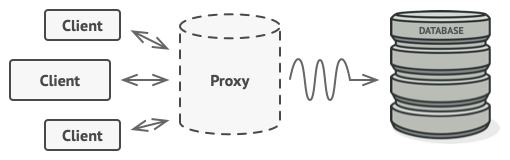
\includegraphics[scale=0.3]{./images/solution.png}
		\end{column}
	
		\begin{column}{.5\textwidth}
			\begin{itemize}
				\item A new proxy class with the same interface as an original service object.
				\item Then you update your app so that it passes the proxy object to all of the original object’s clients.
				\item Upon receiving a request from a client, the proxy creates a real service object and delegates all the work to it.
			\end{itemize}
		\end{column}
	\end{columns}
\end{frame}

\begin{frame}{The Intent of Proxy Design Pattern}
	\begin{center}
	\textcolor{red}{\textbf{Proxy is a structural design pattern that lets you provide a substitute or placeholder for another object. A proxy controls access to the original object, allowing you to perform something either before or after the request gets through to the original object.}}\\
	\end{center}
\end{frame}

\begin{frame}{Structure of proxy Pattern}
	\begin{center}
	\begin{tikzpicture}
 	\umlemptyclass[x=0,y=0]{Client}
 	\umlclass[x=3,y=0]{Subject}{}{request()}
 	\umlclass[x=0,y=-5]{Proxy}{}{request()}
 	\umlclass[x=9,y=-5]{RealObject}{}{request()}
 	\umluniassoc[pos=0.95, align=right, name=uniassoc]{Client}{Subject}
 	\umluniassoc[pos=0.95, align=right, name=uniassoc]{Proxy}{RealObject}
 	\umlinherit[geometry=|-|, pos=0.95, align=right, name=uniassoc]{Proxy}{Subject}
	\end{tikzpicture}	
	\end{center}
\end{frame}

\begin{frame}{Structure of proxy Pattern}
	\begin{itemize}
		\setlength\itemsep{1em}
		\item  The Service Interface declares the interface of the Service. The proxy must follow this interface to be able to disguise itself as a service object.
		\item The Service is a class that provides some useful business logic.
		\item The Proxy class has a reference field that points to a service object. After the proxy finishes its processing (e.g., lazy initialization, logging, access control, caching, etc.), it passes the request to the service object.
		\item Usually, proxies manage the full lifecycle of their service objects.
		\item The Client should work with both services and proxies via the same interface. This way you can pass a proxy into any code that expects a service object.
	\end{itemize}
\end{frame}

\begin{frame}{Applicability}
	\begin{itemize}
		\setlength\itemsep{1em}
		\item Lazy initialization (virtual proxy). This is when you have a heavyweight service object that wastes system resources by being always up, even though you only need it from time to time.
		% Instead of creating the object when the app launches, you can delay the object’s initialization to a time when it’s really needed.
		\item Access control (protection proxy). This is when you want only specific clients to be able to use the service object; for instance, when your objects are crucial parts of an operating system and clients are various launched applications (including malicious ones).
		% The proxy can pass the request to the service object only if the client’s credentials match some criteria.
		\item Local execution of a remote service (remote proxy). This is when the service object is located on a remote server.
		% In this case, the proxy passes the client request over the network, handling all of the nasty details of working with the network.
		\item Logging requests (logging proxy). This is when you want to keep a history of requests to the service object.
		% The proxy can log each request before passing it to the service.
	\end{itemize}
\end{frame}

\begin{frame}{Applicability}
	\begin{itemize}
		\setlength\itemsep{1em}
		\item Caching request results (caching proxy). This is when you need to cache results of client requests and manage the life cycle of this cache, especially if results are quite large.
		% The proxy can implement caching for recurring requests that always yield the same results. The proxy may use the parameters of requests as the cache keys.
		\item Smart reference. This is when you need to be able to dismiss a heavyweight object once there are no clients that use it.
		% The proxy can keep track of clients that obtained a reference to the service object or its results. From time to time, the proxy may go over the clients and check whether they are still active. If the client list gets empty, the proxy might dismiss the service object and free the underlying system resources.
		% The proxy can also track whether the client had modified the service object. Then the unchanged objects may be reused by other clients.
	\end{itemize}
\end{frame}

\begin{frame}{How to Implement}
	\begin{itemize}
		\setlength\itemsep{1em}
		\item If there’s no pre-existing service interface, create one to make proxy and service objects interchangeable. Extracting the interface from the service class isn’t always possible, because you’d need to change all of the service’s clients to use that interface. Plan B is to make the proxy a subclass of the service class, and this way it’ll inherit the interface of the service.
		\item Create the proxy class. It should have a field for storing a reference to the service. Usually, proxies create and manage the whole life cycle of their services. On rare occasions, a service is passed to the proxy via a constructor by the client.
		\item Implement the proxy methods according to their purposes. In most cases, after doing some work, the proxy should delegate the work to the service object.
		\item Consider introducing a creation method that decides whether the client gets a proxy or a real service. This can be a simple static method in the proxy class or a full-blown factory method.
		\item Consider implementing lazy initialization for the service object.
	\end{itemize}
\end{frame}

\begin{frame}{Pros and Cons}
	\begin{columns}[T]
		\begin{column}{.5\textwidth}
			\begin{itemize}
				\item You can control the service object without clients knowing about it.
				\item You can manage the lifecycle of the service object when clients don’t care about it.
				\item The proxy works even if the service object isn’t ready or is not available.
				\item Open/Closed Principle. You can introduce new proxies without changing the service or clients.
			\end{itemize}
		\end{column}
	
		\begin{column}{.5\textwidth}
			\begin{itemize}
				\item The code may become more complicated since you need to introduce a lot of new classes.
				\item The response from the service might get delayed.
			\end{itemize}
		\end{column}
	\end{columns}
\end{frame}

\begin{frame}{Relations with Other Patterns}
	\begin{itemize}
		\setlength\itemsep{1em}
		\item Adapter provides a different interface to the wrapped object, Proxy provides it with the same interface, and Decorator provides it with an enhanced interface.
		\item Facade is similar to Proxy in that both buffer a complex entity and initialize it on its own. Unlike Facade, Proxy has the same interface as its service object, which makes them interchangeable.
		\item Decorator and Proxy have similar structures, but very different intents. Both patterns are built on the composition principle, where one object is supposed to delegate some of the work to another. The difference is that a Proxy usually manages the life cycle of its service object on its own, whereas the composition of Decorators is always controlled by the client.
	\end{itemize}
\end{frame}

\begin{frame}
\begin{center}
{\fontsize{40}{50}\selectfont Thank You!}
\end{center}
\end{frame}

\end{document}
